\subsection{Representation Engineering}
\label{sec:representation_engineering}

\begin{figure}[htbp]
\centering
% Width uses \textwidth; height auto-scales with !
\resizebox{\textwidth}{!}{%
\begin{tikzpicture}
% --- 1. Define leaf nodes (papers, citations added) ---
\node[leaf] (safety_papers) {
InferAligner~\citep{Wang2024InferAligner}, O'Brien et al.~\citep{OBrien2024SAERefusal}, Arditi et al.~\citep{Arditi2024SingleDirection}, CAST~\citep{Lee2024CAST}, AlphaSteer~\citep{Sheng2025AlphaSteer}, Zhou et al.~\citep{zhou2024role}, DRO~\citep{zheng2024prompt}, SafeSwitch~\citep{han2025safeswitch}, Gao et al.~\citep{gao-etal-2025-shaping}, Latent Guard~\citep{zhao2025llms}.
};
\node[leaf, below=0.3cm of safety_papers] (factuality_papers) {
ITI~\citep{li2023iti}, NL-ITI~\citep{hoscilowicz2024nliti}, LITO~\citep{bayat2024enhanced}, ACT~\citep{wang2024act}, Liu et al.~\citep{liu2024uth}, Li et al.~\citep{li2025truthneurons}.
};
\node[leaf, below=0.3cm of factuality_papers] (fairness_papers) {
FairSteer~\citep{Li2025FairSteer}, INLP~\citep{Ravfogel2020INLP}, LEACE~\citep{Belrose2023LEACE}, TaCo~\citep{Jourdan2024TaCo}, Sent-Debias~\citep{Liang2020SentDebias}.
};
\node[leaf, below=0.3cm of fairness_papers] (privacy_papers) {
Nakka et al.~\citep{nakka2025piijailbreaking}, Suri et al.~\citep{suri2025mitigatingmemorization}.
};
% --- 2. Define main sub-nodes (Trustworthiness dimensions) ---
% Positioned to the left of corresponding leaf nodes
\node[sub, left=0.5cm of safety_papers] (safety) {Safety};
\node[sub, left=0.5cm of factuality_papers] (factuality) {Factuality \& Faithfulness};
\node[sub, left=0.5cm of fairness_papers] (fairness) {Fairness};
\node[sub, left=0.5cm of privacy_papers] (privacy) {Privacy};
% --- 3. Define root node ---
% Use the calc library to vertically center the root node relative to the sub-nodes
\node[main, left=2.5cm of {$(safety.west)!0.5!(privacy.west)$}] (repe) {Representation Engineering (§\ref{sec:representation_engineering})};
% --- 4. Draw connection lines ---
% a. Draw a main trunk from the root node to a branching point
\coordinate (fork) at ($(repe.east)+(1.25cm,0)$);
\draw[line] (repe.east) -- (fork);
% b. Connect from main branching point to each sub-node
\draw[line] (fork) |- (safety.west);
\draw[line] (fork) |- (factuality.west);
\draw[line] (fork) |- (fairness.west);
\draw[line] (fork) |- (privacy.west);
% c. Connect main sub-nodes directly to leaf nodes
\draw[line] (safety.east) -- (safety_papers.west);
\draw[line] (factuality.east) -- (factuality_papers.west);
\draw[line] (fairness.east) -- (fairness_papers.west);
\draw[line] (privacy.east) -- (privacy_papers.west);
\end{tikzpicture}%
}
\caption{A taxonomy of Representation Engineering for enhancing LLM trustworthiness.}
\label{fig:repe_taxonomy}
\end{figure}

% \subsubsection{Core Principle: Intervening in the Model's Computational Path}
% Defines Representation Engineering (Activation Steering) as the targeted modification of internal activations during inference to guide high-level conceptual outputs without altering weights.

\subsubsection{Core Principle}
Representation Engineering (RepE) is an inference-time control paradigm for LLMs that directly modifies internal activations, often in the residual stream at selected layers, to steer high-level behaviors such as refusal~\citep{zheng2024prompt, gao-etal-2025-shaping} or truthfulness~\citep{li2023iti}. Unlike methods that focus on individual neurons or fully specified circuits, RepE treats concepts as directions or low-rank subspaces in population activations and manipulates them directly. This top-down view supports both probing and steering of abstract properties within a single forward pass~\citep{zou2023representation}. In practice, RepE identifies how a concept is encoded in activations, represents it as a direction or subspace, and applies targeted control through activation steering or related interventions. This makes RepE a flexible, efficient, and interpretable way to shape model behavior while largely preserving overall capabilities~\citep{wehner2025taxonomy}.

\begin{figure*}[htbp]
  \centering
  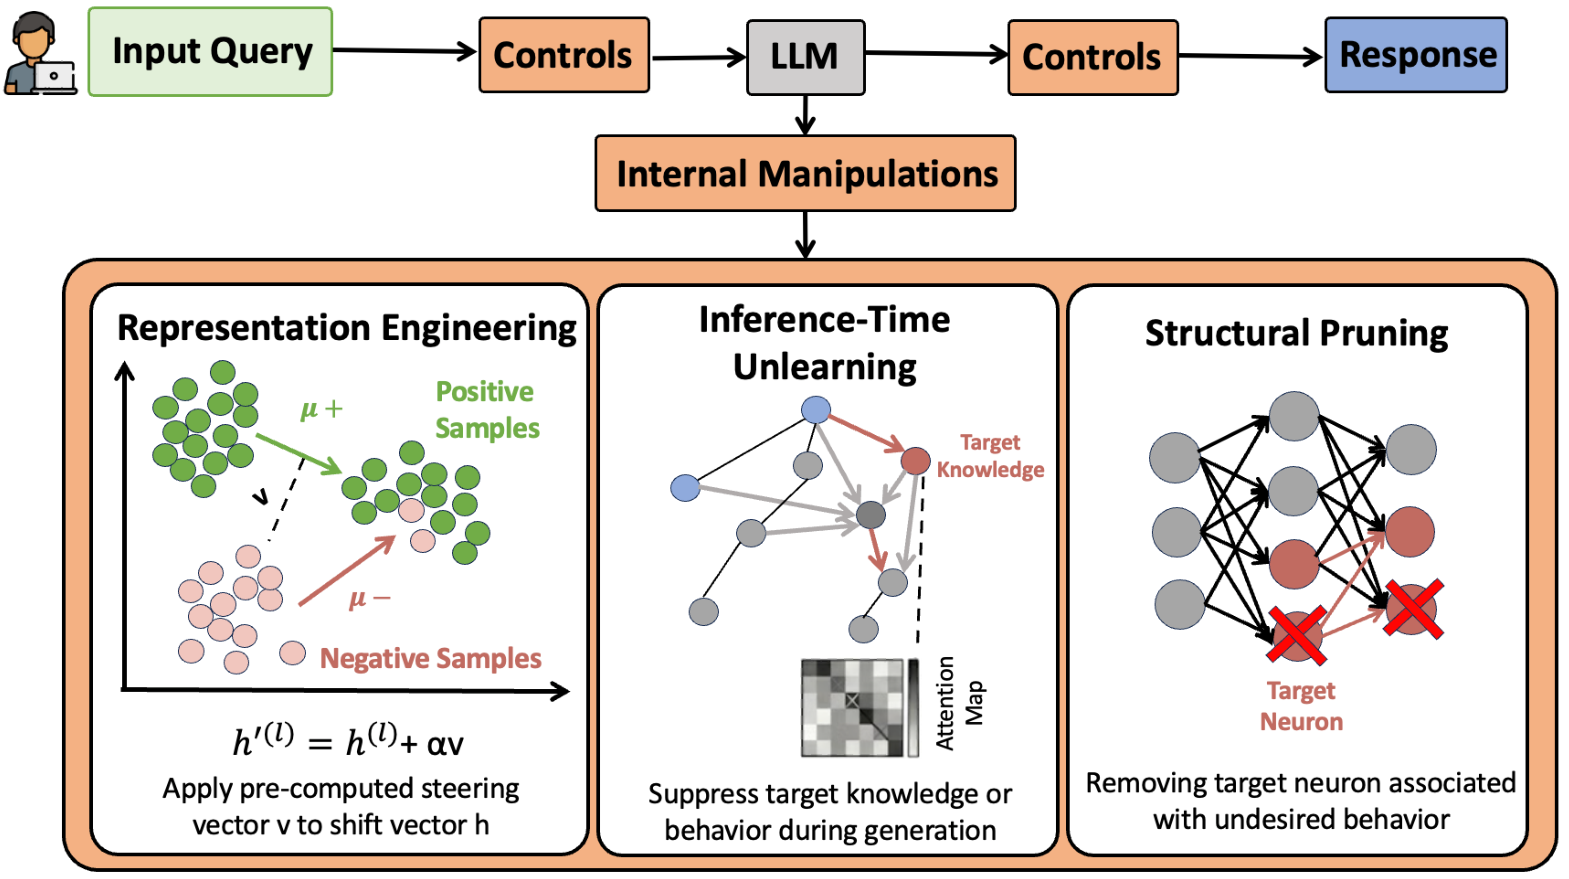
\includegraphics[width=0.85\linewidth]{figures/method/steering_unlearning_pruning.pdf}
  \caption{Overview of internal manipulation methods at inference time, including representation engineering, inference-time unlearning, and structure-level interventions such as pruning.}
  \label{fig:method_unlearning_editing_steering}
\end{figure*}


% Explains the process of creating steering vectors via activation differencing on contrasting prompts and applying them during inference.

% \subsubsection{The Mechanism: Crafting and Applying Steering Vectors}
% The core mechanism of RepE relies on the construction of steering vectors-linear operators defined in the model’s activation space-that capture semantic directions associated with specific concepts. The process unfolds in two steps: identifying concept-relevant representations and applying them during inference.

% Formally, let $h^{(\ell)} \in \mathbb{R}^d$ denote the hidden representation at layer $\ell$ in the residual stream of a transformer model, where $d$ is the dimensionality of the representation space. Given two sets of input prompts, $X^{+}$ (positive examples exhibiting a target concept, e.g., truthful answers) and $X^{-}$ (negative examples, e.g., untruthful answers), we obtain their mean activations at a chosen layer:
% \begin{equation}
% \mu^{+} = \frac{1}{|X^{+}|} \sum_{x \in X^{+}} h^{(\ell)}(x), 
% \qquad 
% \mu^{-} = \frac{1}{|X^{-}|} \sum_{x \in X^{-}} h^{(\ell)}(x).
% \end{equation}

% The \emph{steering vector} $v$ is then defined as the contrastive direction:
% \begin{equation}
% v = \mu^{+} - \mu^{-}.
% \end{equation}

% This vector $v$ operationalizes the concept as a linear direction in activation space. More generally, one may apply dimensionality reduction (e.g., PCA~\citep{Jolliffe:1986}, SVD~\citep{Golub1971}, SAE~\citep{makhzani2013k, cunningham2023sparse}) or optimization-based methods to extract low-rank subspaces $V \subseteq \mathbb{R}^d$ that encode the concept beyond a single direction~\citep{10.1109/TPAMI.2012.88, elhamifar2013sparse, jiang2025msrs, turner2023steering, zhou2025compositional}.

% At inference time, steering is performed by modifying the residual stream activation before it is passed to subsequent layers. For an input $x$ producing hidden state $h^{(\ell)}(x)$, the steered representation is:
% \begin{equation}
% \tilde{h}^{(\ell)}(x) = h^{(\ell)}(x) + \alpha v,
% \end{equation}
% where $\alpha \in \mathbb{R}$ is a control parameter that governs the intensity and polarity of the intervention. Positive values of $\alpha$ amplify the target concept, while negative values suppress it.

% This linear modification is computationally efficient, as it introduces no additional parameters or inference-time cost beyond a single vector addition. Moreover, by tuning $\alpha$ dynamically, one can continuously adjust model behavior without retraining or modifying weights~\citep{turner2023steering}. Extensions of this approach include affine transformations of the form
% \begin{equation}
% \tilde{h}^{(\ell)}(x) = W h^{(\ell)}(x) + b,
% \end{equation}
% where $(W, b)$ are learned steering operators constrained to be low-rank, offering more expressive yet still efficient forms of control~\citep{krasheninnikov2024steering, nguyen-etal-2025-multi,  jiang2025msrs, zhou2025compositional}.

\subsubsection{Mechanism}
RepE typically works by constructing steering vectors, which are directions in activation space associated with a target concept, and injecting them during inference. This process has two stages: identifying concept-relevant representations and applying them at selected layers.

Let $h^{(\ell)} \in \mathbb{R}^d$ denote the hidden representation at layer $\ell$ in the residual stream, where $d$ is the representation dimension. Given two prompt sets, $X^{+}$ for the target concept and $X^{-}$ for its contrast, we compute their mean activations at layer $\ell$:
\[
\mu^{+} = \frac{1}{|X^{+}|} \sum_{x \in X^{+}} h^{(\ell)}(x),
\qquad
\mu^{-} = \frac{1}{|X^{-}|} \sum_{x \in X^{-}} h^{(\ell)}(x).
\]
The steering vector is then defined as
\[
v = \mu^{+} - \mu^{-},
\]
representing the concept as a direction in activation space. More generally, dimensionality reduction methods such as PCA~\citep{Jolliffe:1986}, SVD~\citep{Golub1971}, and SAE, as well as optimization-based methods, can be used to extract low-rank subspaces that capture the concept beyond a single direction~\citep{jiang2025msrs, turner2023steering, zhou2025compositional}.

During inference, the model is steered by modifying the residual activation before it is passed to later layers. For an input $x$ with hidden state $h^{(\ell)}(x)$, the steered representation is
\[
\tilde{h}^{(\ell)}(x) = h^{(\ell)}(x) + \alpha v,
\]
where $\alpha \in \mathbb{R}$ controls the strength and direction of the intervention. Positive $\alpha$ strengthens the target concept, while negative $\alpha$ suppresses it. This intervention is lightweight because it adds no trainable parameters and only requires a vector addition at inference time. By adjusting $\alpha$, model behavior can be continuously controlled without retraining or weight updates~\citep{turner2023steering}. Some extensions replace the additive form with affine transformations,
\[
\tilde{h}^{(\ell)}(x) = W h^{(\ell)}(x) + b,
\]
where $(W, b)$ are low-rank steering operators that provide more expressive but still efficient control~\citep{jiang2025msrs, zhou2025compositional}.




% \subsubsection{Applications in Trustworthiness Dimensions}
% \paragraph{Safety}
% Representation engineering has become a core tool in AI safety research, spanning both the analysis of safety-relevant concepts in internal representations and the use of vector steering to modulate model outputs. Recent work converges on \emph{inference-time} control of internal states. InferAligner introduces cross-model guidance, injecting safety steering vectors during generation to curb harmful completions without sacrificing utility~\citep{Wang2024InferAligner}. Category-wise steering extends this idea with harm-specific vectors, enabling finer-grained, modular control~\citep{Bhattacharjee2024CategorySteer}. A complementary line leverages sparse autoencoders: one thread identifies refusal-mediating features and shows that amplifying them improves robustness, albeit with potential trade-offs in general capability~\citep{OBrien2024SAERefusal}; another uses SAE-derived directions to detoxify outputs with tunable aggressiveness~\citep{Goyal2025BreakingBadTokens}. Mechanistic studies reveal that refusal is largely governed by a single linear direction, motivating targeted interventions~\citep{Arditi2024SingleDirection}. Building on this, runtime methods adjust a sparse subset of hidden states to balance safety and utility on the fly~\citep{Shen2024JailbreakAntidote}, and conditional activation steering triggers refusals only under specific semantic conditions~\citep{Lee2024CAST}. Finally, to mitigate \emph{false} refusals, single-vector ablation surgically removes a ``false-refusal'' direction, preserving helpfulness while maintaining safety~\citep{Wang2024FalseRefusalAblation}, and AlphaSteer learns a principled refusal vector with a null-space constraint to minimize impact on benign prompts~\citep{Sheng2025AlphaSteer}. Together, these approaches constitute a practical toolkit for activation-level safety control that is lightweight, interpretable, and increasingly precise. A recent study~\citep{zhou2024role} also identifies specific ``safety attention heads'' in LLMs---quantified via a Safety Head Important Score (Ships) and located by the Sahara algorithm---showing that ablating just one such head can substantially degrade safety (e.g., yielding up to 16$\times$ more harmful responses) with minimal parameter change.

% Zheng et al.~\citep{zheng2024prompt} show that generic safety prompts tend to push inputs in representation space toward a ``higher-refusal'' direction, increasing blanket refusals \textit{even though LLMs can already distinguish harmful from harmless queries}. They introduce DRO, which optimizes continuous safety prompts to \emph{selectively} steer harmful queries toward refusal. Inspired by this, subsequent studies propose both stronger jailbreak methods and more robust defenses against adversarial attacks~\citep{han2025safeswitch, huang2024jailbreaking, gao-etal-2025-shaping, cao2025scans, 10.1145/3701716.3717659, 10.1145/3627673.3679821, zhao2025llms}. For example, Huang et al. exploit ambiguity near the harmful/harmless boundary, transforming inputs to evade safeguards~\citep{huang2024jailbreaking}. Zhao et al. further show that harmfulness and refusal correspond to distinct latent directions, enabling mechanisms like Latent Guard for more robust safety control~\citep{zhao2025llms}. This line of work provides a sharper mechanistic lens on how attention heads and latent directions contribute to safe behavior.

\subsubsection{Applications}
\paragraph{Safety}
Representation engineering has become an important tool for safety control at inference time. Existing work mainly uses activation-level steering to modulate refusals, suppress harmful outputs, or reduce false refusals. Some methods inject safety vectors during generation, either through cross-model guidance or harm-specific steering, to improve safety while preserving utility~\citep{Wang2024InferAligner}. Others use sparse autoencoders to identify refusal-related features or derive steering directions for detoxification, which improves controllability but may introduce utility trade-offs~\citep{OBrien2024SAERefusal}. Mechanistic studies further suggest that refusal behavior can often be traced to a small set of latent directions or attention components, which enables more targeted interventions such as conditional activation steering and false-refusal ablation~\citep{Arditi2024SingleDirection, Lee2024CAST, Sheng2025AlphaSteer, zhou2024role}.

This line of work also provides a clearer view of how safety steering interacts with jailbreak robustness. Prior studies show that generic safety prompts often over-shift representations toward refusal, which can increase blanket refusals even when the model can distinguish harmful from benign inputs~\citep{zheng2024prompt}. In response, later methods study more selective steering strategies and more robust safety control under adversarial prompting~\citep{han2025safeswitch, gao-etal-2025-shaping, zhao2025llms}. Overall, these results show that representation engineering offers a lightweight and increasingly precise toolkit for inference-time safety control.


\paragraph{Fairness}
% Identifies the lack of dedicated research and theorizes potential applications.
Fairness can also be improved through interventions on internal representations rather than full retraining. In inference-time settings, activation steering uses bias-related directions to modify hidden states and reduce demographic or ideological skew. Recent methods further adapt the intervention layer and strength to improve fairness with limited utility loss~\citep{Li2025FairSteer}. Related work studies concept erasure, which removes protected-attribute information from embeddings or activations through projection or transformation. Representative methods include INLP, LEACE, TaCo, and Sent-Debias~\citep{Ravfogel2020INLP, Belrose2023LEACE, Jourdan2024TaCo, Liang2020SentDebias}. Together, these studies suggest that representation-level interventions can help reduce bias without full model retraining.

% A growing line of work shows that fairness can be improved by directly editing a model’s internal representations rather than retraining full models. On the inference-time side, \emph{activation steering} computes bias-directed vectors and adds or subtracts them to hidden states to reduce demographic or ideological skew; recent methods dynamically select layers and strengths, delivering debiasing with minimal utility loss~\citep{Li2025FairSteer, Siddique2025SteeringVectors, Nadeem2025SteeringFairness}. Complementary \emph{concept-erasure} approaches remove protected-attribute information from embeddings or activations. Early linear techniques, such as Iterative Nullspace Projection (INLP) and linear adversarial erasure project out subspaces predictive of gender/race and can be applied to contextual encoders~\citep{Ravfogel2020INLP}. LEACE provides a closed-form transformation that provably eliminates all \emph{linear} detectability while minimally altering features, and can be layered into ``concept scrubbing'' across networks~\citep{Belrose2023LEACE}. To protect against \emph{nonlinear} recovery, targeted concept-erasure methods (e.g., TaCo) rank and remove latent concepts to block sensitive-attribute leakage from nonlinear probes~\citep{Jourdan2024TaCo}. At the sentence level, Sent-Debias extends projection-based removal to contextual representations~\citep{Liang2020SentDebias}. Finally, model-editing based debiasing (e.g., BIASEdit) performs lightweight parameter edits guided by representation probes, offering another practical axis of fairness-oriented representation engineering~\citep{Xu2025BiasEdit}.




\paragraph{Privacy}
% Both mitigating memorization by steering away from private data and inducing privacy leaks by steering towards it.
Representation engineering also plays a dual role in privacy, as activation steering can both expose and mitigate leakage. On the attack side,~\citet{nakka2025piijailbreaking} identify refusal-related attention heads for sensitive attributes and steer a small subset of them at inference time to bypass safeguards, leading to high disclosure rates across several LLMs. On the defense side,~\citet{suri2025mitigatingmemorization} show that activation steering can suppress verbatim memorization on a controlled benchmark with limited quality loss. Together, these results suggest that inference-time steering can serve both privacy auditing and mitigation without retraining.

% Discusses its use in steering models towards harmlessness.

\paragraph{Factuality and Faithfulness}

A major line of work in representation engineering steers internal activations at inference time to improve truthfulness without updating model weights. ITI shifts a small set of attention-head activations along truth-related directions and substantially improves TruthfulQA accuracy on Alpaca~\citep{li2023iti}. NL-ITI extends this idea with multi-token non-linear interventions and reports further gains over ITI~\citep{hoscilowicz2024nliti}. To avoid fixed intervention strengths, LITO learns an instance-specific schedule and can back off through uncertainty-aware refusal, improving truthfulness while preserving task accuracy~\citep{bayat2024enhanced,bayat2024enhanced}. ACT learns a bank of steering vectors and adapts intervention strength by hallucination category, showing gains across the LLaMA family~\citep{wang2024act}. Other studies provide a more mechanistic view by identifying global truth-related structure in representation space or finer-grained truth neurons associated with truthful output~\citep{liu2024uth, li2025truthneurons}. 

% Explores steering towards "truthfulness" to mitigate hallucinations, questioning whether complex knowledge can be controlled by low-rank interventions.
% A consistent thread in representation engineering is to \emph{steer} internal activations at inference time to elicit truth, without updating weights. Linear ITI shifts a small set of attention-head activations along “truth” directions and roughly doubles TruthfulQA accuracy on Alpaca~\citep{li2023iti}. NL-ITI replaces linear probing with multi-token, non-linear interventions and reports further gains on TruthfulQA over the ITI baseline~\citep{hoscilowicz2024nliti}. To avoid brittle, one-size-fits-all strengths, LITO learns an instance-specific intervention schedule and backs off via uncertainty-aware refusal, improving truthfulness while preserving task accuracy~\citep{bayat2024enhanced,bayat2024enhanced}. ACT learns a bank of steering vectors and adapts strength by hallucination category, yielding improvements across the LLaMA family~\citep{wang2024act}. Geometrically, evidence for a universal “truthfulness hyperplane” suggests globally structured truth signals inside LLMs~\citep{liu2024uth}; at a finer granularity, \emph{truth neurons}—units predictive of truthful vs.\ untruthful output—have been identified, and suppressing them degrades performance across benchmarks~\citep{li2025truthneurons}. Together, these results indicate that inference-time representation interventions can systematically improve factuality/faithfulness without retraining.





% \subsubsection{Discussion: Granularity, Strengths, and Fundamental Challenges}
% Strengths: Fine-grained control over high-level, abstract properties.
% Limitations: Vectors are rarely conceptually "pure," risk of out-of-distribution behavior, and interventions are often model-specific and empirical.

% Representation engineering conceptualizes hidden states as controllable objects for identifying, operationalizing, and steering internal concepts, complementing prompting and parameter-efficient finetuning while advancing transparency~\citep{zou2023representation,wehner2025taxonomy,bartoszcze2025survey}. Along the axis of \emph{granularity}, RepE spans (i) direction/concept-level editing via inference-time intervention and activation addition~\citep{li2023iti,turner2023steering,rimsky2024caa}, including subspace-oriented scaling/finetuning~\citep{stoehr2024activationscaling,wu2024reft} and token- or layer-specific placement; and (ii) feature-level steering with sparse autoencoders that expose interpretable latents~\citep{OBrien2024SAERefusal}. Empirically, SAE studies report encouraging cross-model commonalities but also seed-level instability, underscoring that the choice of features, layers, and normalization critically shapes outcomes~\citep{lan2024universal,paulo2025saeinstability,park2023linear}. 

% The principal \emph{strengths} of RepE are efficiency, modularity, and interpretability. Many methods operate at inference time without weight updates, enabling rapid iteration and composition with prompts and safety guards; representation finetuning (ReFT) and related subspace methods further provide parameter-efficient persistence while keeping base weights intact~\citep{wu2024reft,stoehr2024activationscaling}. Linear composition of concept directions supports multi-attribute control—e.g., truthfulness with low toxicity or calibrated refusal—leveraging category- or condition-specific variants~\citep{li2023iti,rimsky2024caa,OBrien2024SAERefusal}. This tight linkage between controllability and internal geometry facilitates systematic auditing and evaluation, aligning with recent surveys that catalog opportunities and open problems for large language models~\citep{wehner2025taxonomy,bartoszcze2025survey}. 

% Reliability hinges on causal validity when collecting contrastive activations; mismatched roles or confounders can spuriously attribute effects, motivating causal designs and matched comparisons~\citep{deng2025care}. Generalization is fragile: steering strength, intervention location, and normalization can flip outcomes; best-practice work in activation/attribution patching warns that metrics and corruption protocols materially affect conclusions~\citep{zhang2023patching,pham2024activationedit}. Beyond these, recent surveys highlight practical obstacles: steering multiple concepts at once remains brittle due to entangled representations, long-form generation control often degrades over extended outputs, and interventions risk shifting activations off their natural distribution, undermining reliability~\citep{wehner2025taxonomy}. Finally, dual-use risks persist: activation-level edits can both harden and erode safety, interacting with jailbreak tactics and safety prompts in complex ways~\citep{revisiting2025jailbreaking,zheng2024prompt,zhou2024role}; governance guidance therefore recommends treating representation-level controls as part of a broader risk-managed stack~\citep{nist2025ai8001}. Establishing robust, portable RepE thus requires standardized robustness protocols, explicit reporting of intervention granularity (concept/feature, spatial, and strength), and principled integration with safety governance.


